
\documentclass[preprint,12pt]{elsarticle}

\usepackage[spanish]{babel}
\usepackage{amssymb}
\usepackage{graphicx}
\usepackage{lineno}
\usepackage[utf8]{inputenc}
\usepackage{url}
\usepackage{natbib} 
\usepackage{amsmath} 
\usepackage{amssymb} 
\usepackage{float}

\begin{document}
	
	\begin{frontmatter} 

		\title{\huge INFORME DE LABORATORIO 07 INSTALACIÓN DE UNA INSTANCIA DE MICROSOFT SQL SERVER}
		
		\author{Huichi Contreras, Franklin Carlos         	(2016054948)} 
		\address{Escuela Profesional de Ingeniería de Sistemas}
		\address{Universidad Privada de Tacna}
		\address{Tacna, Perú}
		

	\end{frontmatter}

%% INTRODUCION ----------------------------------------------------------------------------------------------------------------

\section{INFORMACIÓN GENERAL} 

\subsection {\textbf{Objetivos}}
\begin{itemize}
	\item Instalación de una instancia SQL Server en Docker y conectarse al mismo mediante SQL Server Management Studio
\end{itemize}

\subsection {\textbf{Equipos, materiales, programas y recursos utilizados}}
\begin{itemize}
	\item Computadora con sistema operativo Windows XP, Vista, Windows 7, Windows 8 y/o Windows 8.1.
	\item CPU SLAT-capable feature al menos 4GB de RAM
	\item Docker Desktop (Para lo cual se debe primero crear una cuenta en Docker Hub)
	\item Microsoft SQL Server Management Studio en su última versión
\end{itemize}

%% ----------------------------------------------------------------------------------------------------------------------------------


%% MARCO TEÓRICO ------------------------------------------------------------------------------------------------------------

\section{Marco Teórico}

%% PRIMERA SUBSECCION 

\subsection {\textbf{Docker}}
Docker se define como un proyecto de código abierto que proporciona una capa de abstracción y virtualización a nivel de sistema operativo, a través de la instalación de contenedores de software.
\subsubsection{\textbf{SQL Server Management Studio}}
SQL Server Management Studio (SSMS) es la interfaz de usuario cliente preferida y oficial con la cual se puede manejar, configurar, desplegar, actualizar y administrar una instancia SQL Server.


\section{PROCEDIMIENTO}

\subsubsection{\textbf{Paso 1: Gestionar Docker Setup}}
\begin{figure}[H]
	\begin{center}
		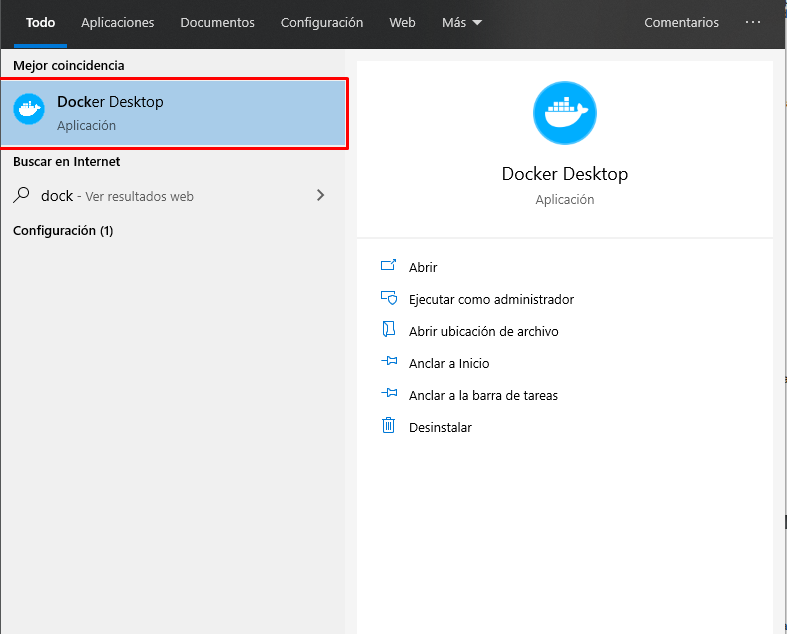
\includegraphics[width=12cm]{./IMAGENES/foto1} 
		\caption{Ingresar a Docker Setup}
	\end{center}
\end{figure}

\begin{figure}[H]
	\begin{center}
		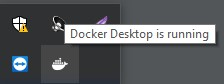
\includegraphics[width=12cm]{./IMAGENES/foto2} 
		\caption{Comprobamos que esta arrancando el Docker}
	\end{center}
\end{figure}

\begin{figure}[H]
	\begin{center}
		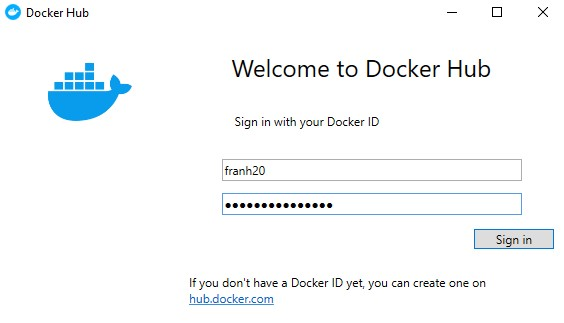
\includegraphics[width=12cm]{./IMAGENES/foto3} 
		\caption{Ingresamos nuestra cuenta de Docker}
	\end{center}
\end{figure}

\begin{figure}[H]
	\begin{center}
		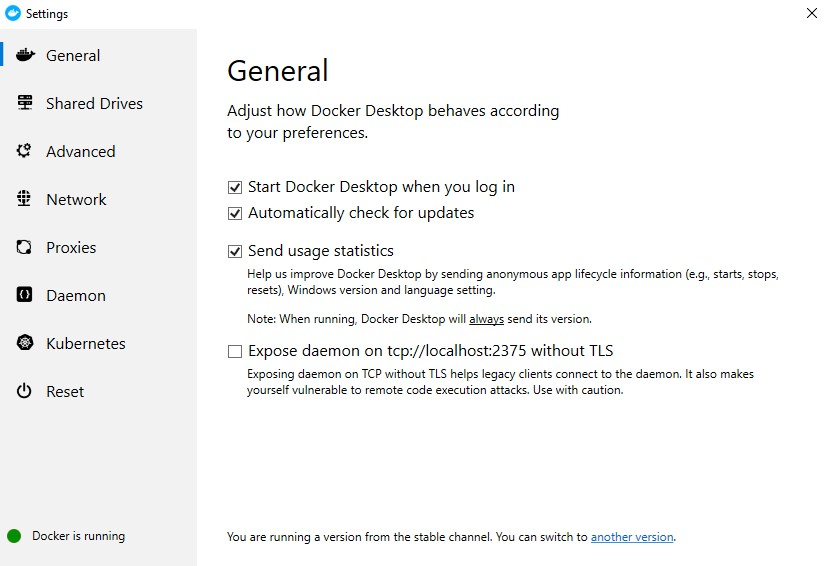
\includegraphics[width=12cm]{./IMAGENES/foto4} 
		\caption{Como se ve podemos ver los ajustes del Docker.}
	\end{center}
\end{figure}

\subsubsection{\textbf{Paso 2: Gestionar los contenedores mediante PowerShell}}

\begin{figure}[H]
	\begin{center}
		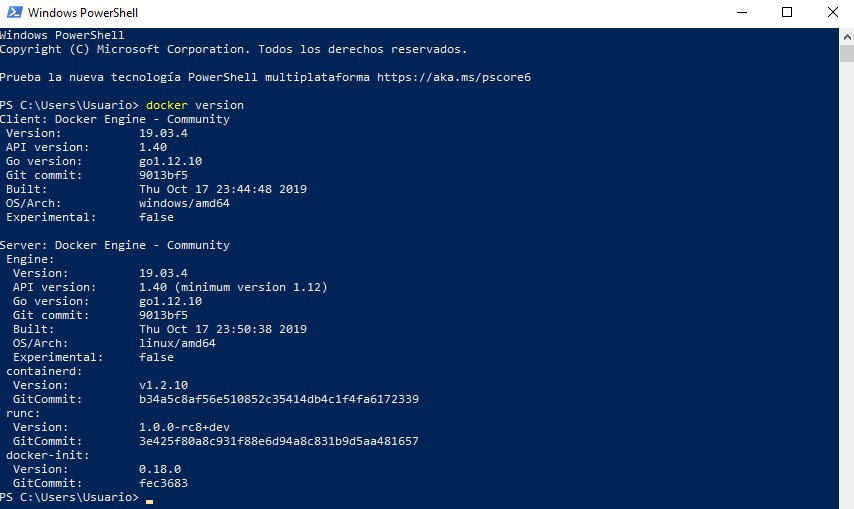
\includegraphics[width=12cm]{./IMAGENES/foto5} 
		\caption{Ingresamos “Docker versión” para ver si tenemos Docker}
	\end{center}
\end{figure}


\begin{figure}[H]
	\begin{center}
		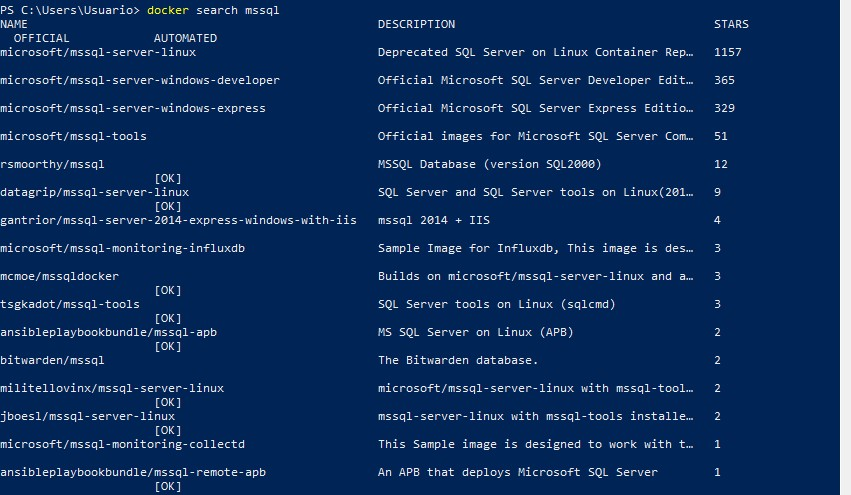
\includegraphics[width=12cm]{./IMAGENES/foto6} 
		\caption{Buscamos la Iso para descargar}
	\end{center}
\end{figure}

\begin{figure}[H]
	\begin{center}
		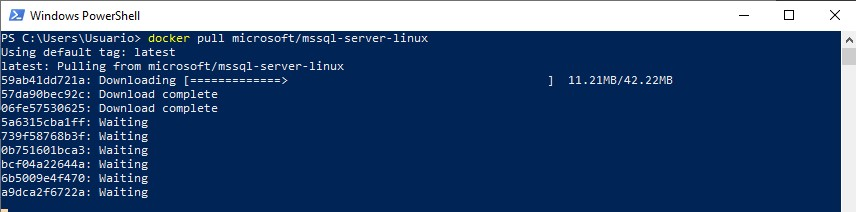
\includegraphics[width=12cm]{./IMAGENES/foto7} 
		\caption{Descargamos la iso definida}
	\end{center}
\end{figure}

\begin{figure}[H]
	\begin{center}
		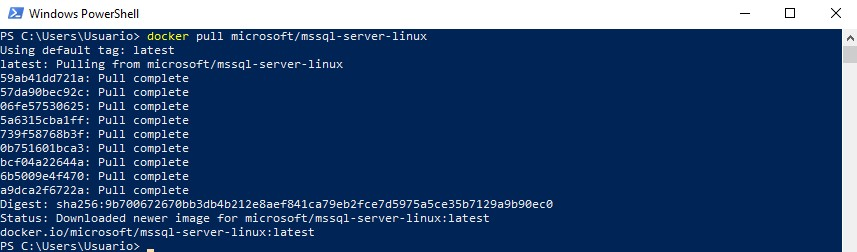
\includegraphics[width=12cm]{./IMAGENES/foto8} 
		\caption{Descargamos la iso definida}
	\end{center}
\end{figure}

\begin{figure}[H]
	\begin{center}
		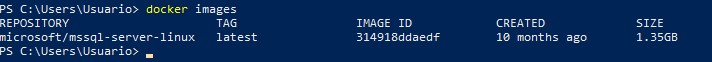
\includegraphics[width=12cm]{./IMAGENES/foto9} 
		\caption{Revisamos si tenemos descargado la ISO}
	\end{center}
\end{figure}

\begin{figure}[H]
	\begin{center}
		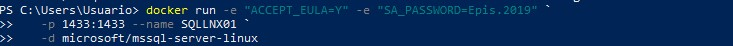
\includegraphics[width=12cm]{./IMAGENES/foto10} 
		\caption{Instalamos nuestro primer contenedor con MSSQL-Server}
	\end{center}
\end{figure}

\begin{figure}[H]
	\begin{center}
		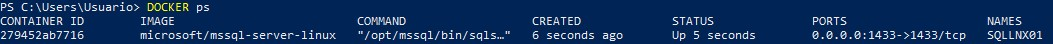
\includegraphics[width=12cm]{./IMAGENES/foto11} 
		\caption{Verificamos que tenemos instalado}
	\end{center}
\end{figure}

\subsubsection{\textbf{Paso 3: Conectarnos a la base de datos mediante Microsoft SQL Server Management Studio}}
\begin{figure}[H]
	\begin{center}
		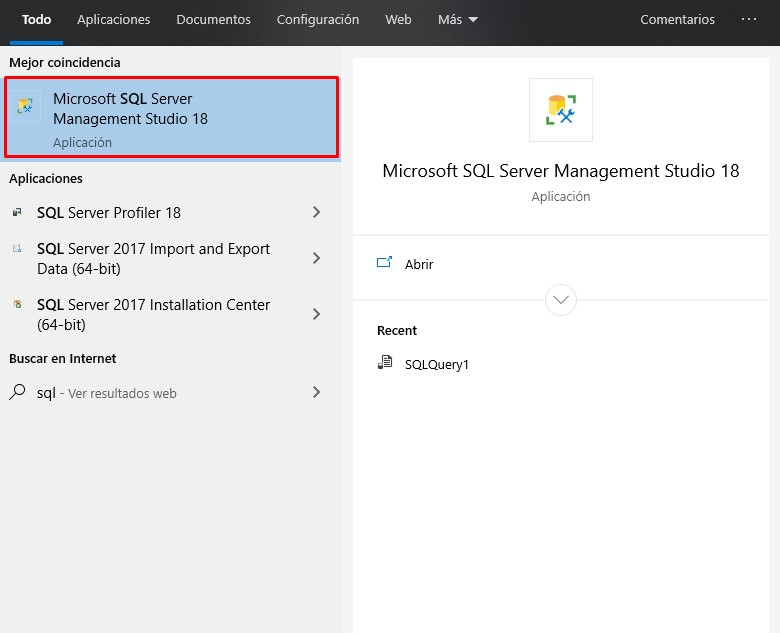
\includegraphics[width=12cm]{./IMAGENES/foto12} 
		\caption{Ingresamos a Management Studio}
	\end{center}
\end{figure}

\begin{figure}[H]
	\begin{center}
		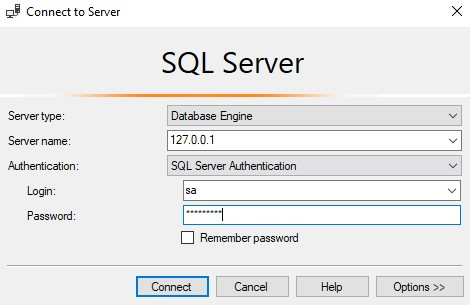
\includegraphics[width=12cm]{./IMAGENES/foto13} 
		\caption{Ingresamos la ip local nuestro cuenta y contraseña establecida al momento de instalación}
	\end{center}
\end{figure}

\begin{figure}[H]
	\begin{center}
		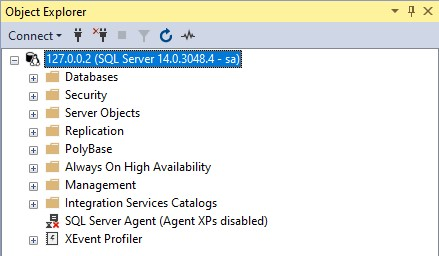
\includegraphics[width=12cm]{./IMAGENES/foto14} 
		\caption{Como podemos visualizar ya nos podemos conectar a nuestra base de datos y visualizar que sale la ID del contenedor}
	\end{center}
\end{figure}

\begin{figure}[H]
	\begin{center}
		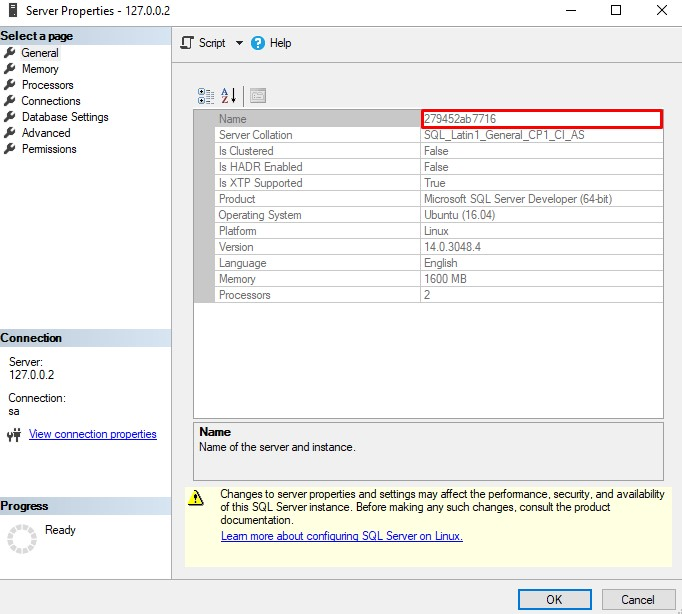
\includegraphics[width=12cm]{./IMAGENES/foto15} 
		\caption{Como podemos visualizar ya nos podemos conectar a nuestra base de datos y visualizar que sale la ID del contenedor}
	\end{center}
\end{figure}

\begin{figure}[H]
	\begin{center}
		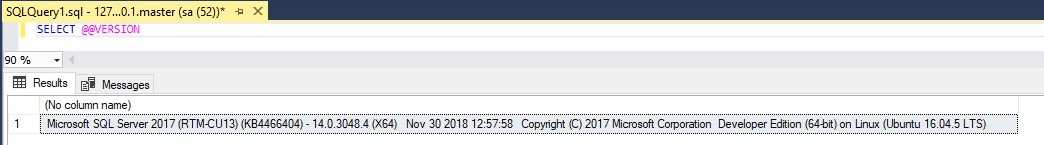
\includegraphics[width=12cm]{./IMAGENES/foto16} 
		\caption{También podemos visualizar nuestra versión}
	\end{center}
\end{figure}

\begin{figure}[H]
	\begin{center}
		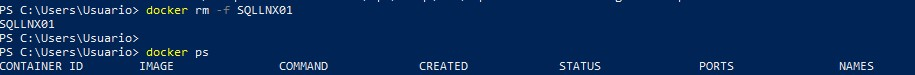
\includegraphics[width=12cm]{./IMAGENES/foto17} 
		\caption{Por último eliminamos nuestra contenedor.}
	\end{center}
\end{figure}

\section{ANALISIS E INTERPRETACION DE RESULTADOS }
\begin{itemize}
	\item ¿Qué indican los resultados? \\
	Pudimos realizar exitosamente la conexión de nuestro contenedor a la base de datos
	\item ¿Que se ha encontrado?\\
	Encontré una manera más rápida de poder tener una base de datos SQL Server sin necesidad de estar haciendo toda la instalación necesaria del MSSQL en mi computadora.
\end{itemize}

\section{CUESTIONARIO}
\begin{itemize}
	\item ¿Con qué comando(s) exportaría la imagen de Docker de Microsoft SQL Server a otra PC o servidor? \\
	Con el comando: docker push Tunombre/my-first-repo
	\item ¿Con qué comando(s) podría generar dos volúmenes para un contenedor para distribuir en un volumen el Archivo de Datos (.mdf) y en otro el Archivo Log (.ldf)?\\
	docker volume create ArchivodeDatos.mdf \\
	docker volume create ArchivodeLog.ldf
	\item Genere un nuevo contenedor y cree la base de datos con las siguientes características.\\
	Nombre : FINANCIERA\\
	Archivos : \\
	DATOS (mdf) : Tamaño Inicial : 50MB, Incremento: 10MB, Ilimitado \\
	INDICES (ndf) Tamaño Inicial : 100MB, Incremento: 20MB, Maximo: 1GB \\
	HISTORICO (ndf) Tamaño Inicial : 100MB, Incremento: 50MB, Ilimitado \\
	LOG (ldf) Tamaño Inicial : 10MB, Incremento: 10MB, Ilimitado \\
	¿Cuál sería el script SQL que generaría esta base de datos?
	
	\begin{figure}[H]
	\begin{center}
		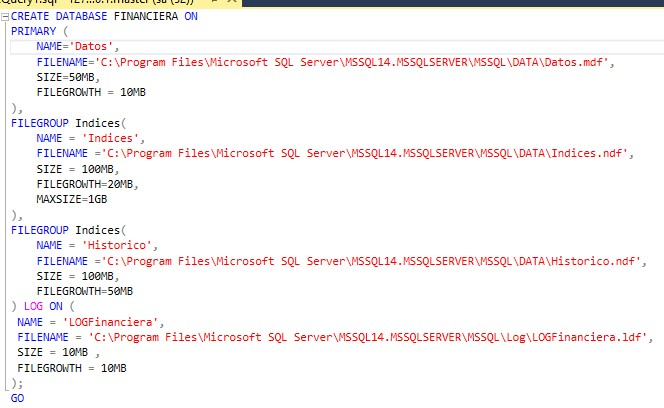
\includegraphics[width=12cm]{./IMAGENES/foto18} 
		\caption{Script planteado}
	\end{center}
	\end{figure}

\end{itemize}

\section{CONCLUSION}
En conclusión, los contenedores nos ayudan a montar nuestra base de datos de forma mas rápida para poder manejar nuestros diversos sistemas a implementarlos y conectarlos, a su vez también aprendí que los ISO nos vienen a permitir con Docker subirlas para poder usarlas en otras ocasiones.

\end{document}
